% Requires running Bibtex

\documentclass[%
reprint,
amsmath,amssymb,
aps,
floatfix
]{revtex4-2}

\usepackage{graphicx}% Include figure files
\usepackage{dcolumn}% Align table columns on decimal point
\usepackage{bm}% bold math
\usepackage{hyperref}% add hypertext capabilities
\usepackage[font=scriptsize,labelfont=bf, justification=justified]{caption}% change fontsize in captions
\usepackage{float}
\usepackage{booktabs}% cool table style
\hypersetup{
	colorlinks=true,       % false: boxed links; true: colored links
	linkcolor=black,        % color of internal links
	citecolor=black,        % color of links to bibliography
	filecolor=black,     % color of file links
	urlcolor=black         
}

\usepackage{listings}

%\usepackage{bibspacing}
%\setlength{\bibitemsep}{.5\baselineskip plus .05\baselineskip minus .05\baselineskip}


\begin{document}
	
	\preprint{APS/123-QED}
	
	\title{PHYC30170 Physics with Astronomy and Space Science Lab 1;\\Electronics}
	
	\author{Daragh Hollman}
	\email{daragh.hollman@ucdconnect.ie}
	
	\date{\today}
	
	\begin{abstract}
		
	\end{abstract}
	
	\maketitle
	
	\section{Introduction}
		Comment on the layout of the exercises and that some are being left out.
	
	\section{Exercise 5: }
		\subsection{Theory}
		What is an RC circuit? What is the expected outcome.\\
		
		Exercise 5 involves the construction and measurement of a RC circuit. An RC circuit is one which consists of a resistor and capacitor. The capacitor stores charge and the resistor controls the rate at which it discharges \cite{pumplin}. This time dependent discharge is an exponential decay given by the following equation:
		\begin{equation}
			V_\text{out} = V_\text{in} \exp{\left(\frac{-t}{RC}\right)}
			\label{eq:expDecay}
		\end{equation}where $V_\text{in}$ is the input voltage and $V_\text{out}$ is the voltage output measured by the voltmeter in figure \ref{fig:sampleRC}. $R$ and $C$ are simply the resistance and capacitance respectively. The factor $1/RC$ is defined as the decay constant which solely determines the rate of decay \cite{manual}.
		
		\begin{figure}
			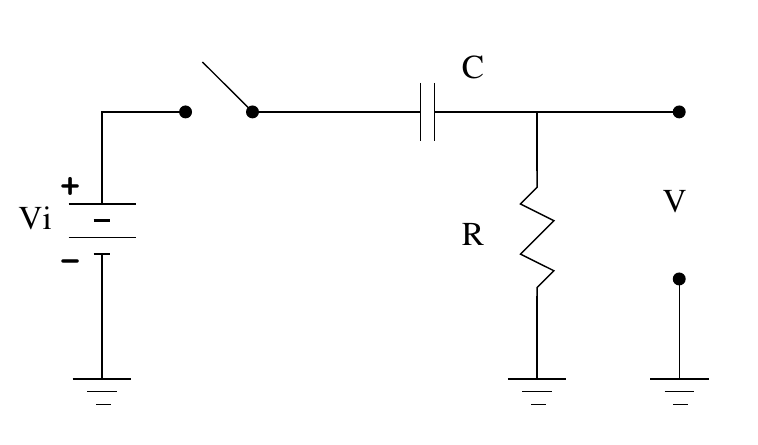
\includegraphics[width=0.85\columnwidth]{sampleRC.png}
			\caption{\label{fig:sampleRC}A sample RC circuit as described in the lab manual \cite{manual}.}
		\end{figure}
	
		\subsection{Methodology}
		The RC circuit depicted in figure \ref{fig:sampleRC} was constructed in DesignSoft's TINA \cite{TINA}, a circuit simulator. This construction is shown in figure \ref{fig:ex5Circuit}. A virtual oscilloscope was used in place of a voltmeter to measure the signal as a function of time. The component values of the capacitor and resistor were chosen as directed by the exercise and a square wave of frequency $20 \,\text{Hz}$ with peak to peak amplitude of $5\,\text{V}$ was used as the input. The circuit was simulated and the signal was recorded. The circuit was then constructed physically on a breadboard and the same measurement was made using an oscilloscope. The signals of the simulation, the measurement, and the analytical solution were then compared and the decay constants determined.
		
		\begin{figure}
			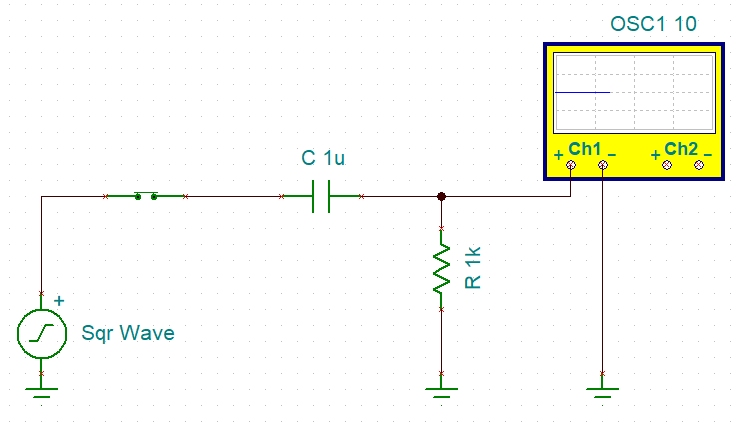
\includegraphics[width=0.85\columnwidth]{circuit_ex5.png}
			\caption{\label{fig:ex5Circuit}The circuit construction created in TINA for simulation.}
		\end{figure}
		
		\subsection{Results \& Analysis}
		The measured data from the breadboard were plotted in figure \ref{fig:ex5Results} along with the analytical solution calculated using equation \ref{eq:expDecay}. The decay constant of the analytical solution was calculated from the values of the resistor and the capacitor however, the decay constants for the measured data and simulation data were determined using least squares fitting of the signal. The decay constants for each method were recorded in table \ref{tab:decayConstants} along with their uncertainty which was determined by the square root of the diagonal elements of the covariance matrix. 
		
		\begin{table}[]
			\resizebox{0.85\columnwidth}{!}{%
				\begin{tabular}{@{}lll@{}}
					\toprule
					Method     & Decay Constant ($s^{-1}$) & Uncertainty \\ \midrule
					Analytical & 1000                    & N/A         \\
					Simulation & 1012.884                 & $\mathcal{O}10^{-6}$           \\
					Measured   & 895.937                  & $\mathcal{O}10^{-6}$           \\ \bottomrule
				\end{tabular}%
			}
			\caption{Decay constants for exercise 5. The uncertainties were determined by the square root of the diagonal elements of the covariance matrix for least squares fitting}
			\label{tab:decayConstants}
		\end{table}
		
	
		\begin{figure}
			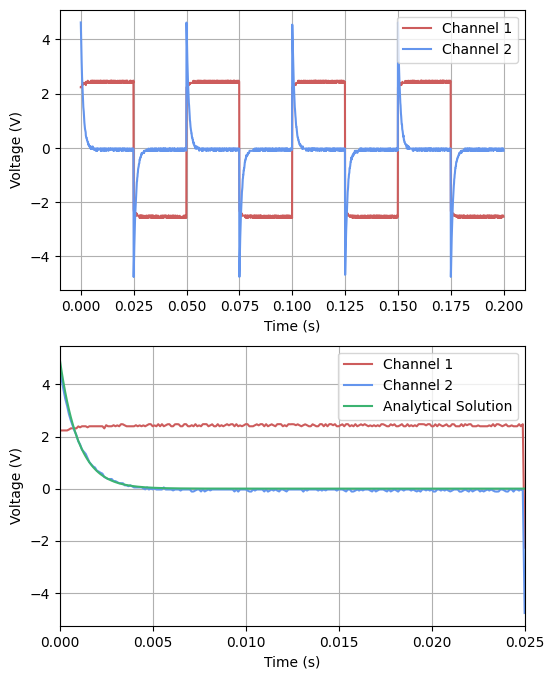
\includegraphics[width=0.85\columnwidth]{ex5_dualPlot.png}
			\caption{\label{fig:ex5Results}Input and output signals from the RC circuit in exercise 5. Channel 1 is the square wave driving the circuit whereas channel 2 is the output. The exponential decay response is clearly shown in the lower graph ($1\over2$ period) in comparison to the analytical solution.}
		\end{figure}
		\begin{figure}
			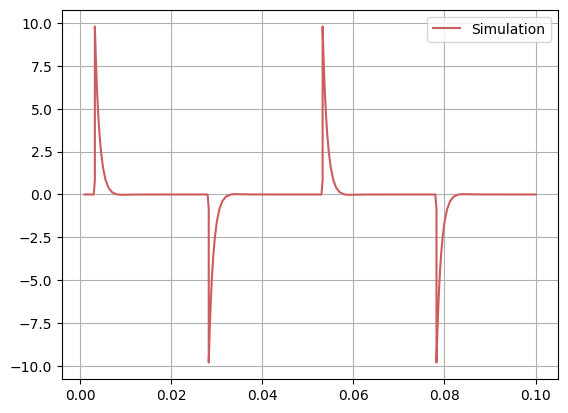
\includegraphics[width=0.85\columnwidth]{ex5_simPlot.png}
			\caption{\label{fig:ex5Sim}Simulation data generated by TINA, is exponential decay the same shape as the analytical and the measured.}
		\end{figure}
		\begin{figure}
			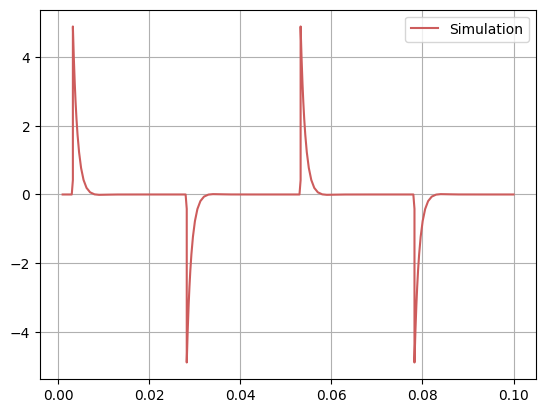
\includegraphics[width=0.85\columnwidth]{ex5_simPlotAdj.png}
			\caption{\label{fig:ex5SimAdj}The simulated data using peak to peak amplitude.}
		\end{figure}
	
		We notice that the amplitude of the simulation data is approximately twice that in the measured data. This is due to an inconsistency in the definition of amplitude, be it peak to peak amplitude or average to peak. We can still see clearly that the shape of the data matches what is expected and therefore dividing by two will yield the result under peak to peak amplitude. This is done explicitly in this exercise as shown in figures \ref{fig:ex5Sim} and \ref{fig:ex5SimAdj} however, for all further exercises where this applies - unless otherwise specified - this can be assumed to have been done.\\
		
		For consistency, in this report we shall use the term amplitude to refer to peak to peak amplitude as this is the definition used by the oscilloscope which was used to generate and measure signals for the majority of these exercises.
		
	\section{Exercise 7: }
		\subsection{Theory}
		Exercise 7 demonstrates how the same RC circuit as in exercise 5 can be used to make a high pass filter \cite{manual}. High pass filter is a signal filter which allows higher frequencies to pass through unaffected but attenuates signals beyond a cut-off frequency. The combination of a resistor with a capacitor makes it possible to have voltage dividers dependent on frequency \cite{horowitz}. This frequency dependence arises from the impedance of the capacitor.
		\begin{equation}
			Z_C = -\frac{j}{\omega C}
		\end{equation}where $j$ is the imaginary number $j=\sqrt{-1}$, $C$ is the capacitance, and $\omega$ is the angular frequency. For the circuit in figure \ref{fig:sampleRC}, by Ohm's law we have a current:
		\begin{equation}
			I = \frac{V_\text{in}}{Z_\text{total}} = \frac{V_\text{in}}{R - Z_C}
		\end{equation}and hence we can calculate the voltage across the resistor, $V_\text{out}$, by substitution and rationalisation of the current:
		\begin{equation}
			V_\text{out} = I R = V_\text{in}\frac{[R+(\frac{j}{\omega C})]R}{R^2 + (\frac{1}{\omega^2 C^2})}
		\end{equation}with a magnitude of:
		\begin{equation}
			V_\text{out} = V_\text{in}\frac{R}{\left[R^2 + \left(\frac{1}{\omega^2 C^2}\right)\right]^\frac{1}{2}} = V_\text{in} \frac{\omega R C}{\left[1 + \left(\omega RC\right)^2\right]^\frac{1}{2}}
		\end{equation}this is derived in full by Horowitz and Hill \cite{horowitz}.
	
	
		\subsection{Methodology}
		\subsection{Results \& Analysis}
		\begin{figure}
			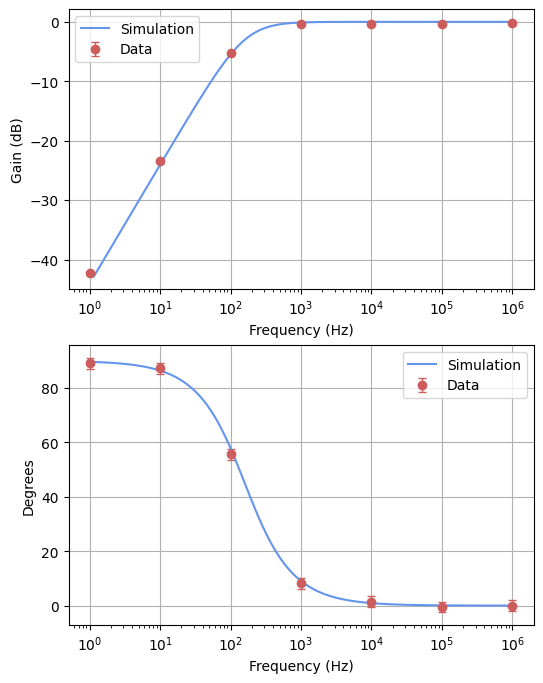
\includegraphics[width=0.85\columnwidth]{ex7_dualPlot.png}
			\caption{\label{fig:ex7Results}Bode plot of exercise 7. The circuit is a high pass filter with $R = 1 \text{k}\Omega$, $C = 1 \mu\text{F}$}
		\end{figure}
		
	\section{Exercise 12: }
		\subsection{Theory}
		\subsection{Methodology}
		\subsection{Results \& Analysis}
		
	\section{Exercise 19: }
		\subsection{Theory}
		\subsection{Methodology}
		\subsection{Results \& Analysis}
	
	\section{Exercise 20: }
		\subsection{Theory}
		\subsection{Methodology}
		\subsection{Results \& Analysis}
		
	\section{Exercise 21: }
		\subsection{Theory}
		\subsection{Methodology}
		\subsection{Results \& Analysis}
		
	\section{Exercise 25: }
		\subsection{Theory}
		\subsection{Methodology}
		\subsection{Results \& Analysis}
		
	\section{Exercise 27: }
		\subsection{Theory}
		\subsection{Methodology}
		\subsection{Results \& Analysis}
		
	\clearpage
	\bibliography{electronics.bib}% Produces the bibliography via BibTeX.
	
	\clearpage
	\onecolumngrid
	\appendix

	
	
\end{document}

